\begin{figure}[t]
\centering
  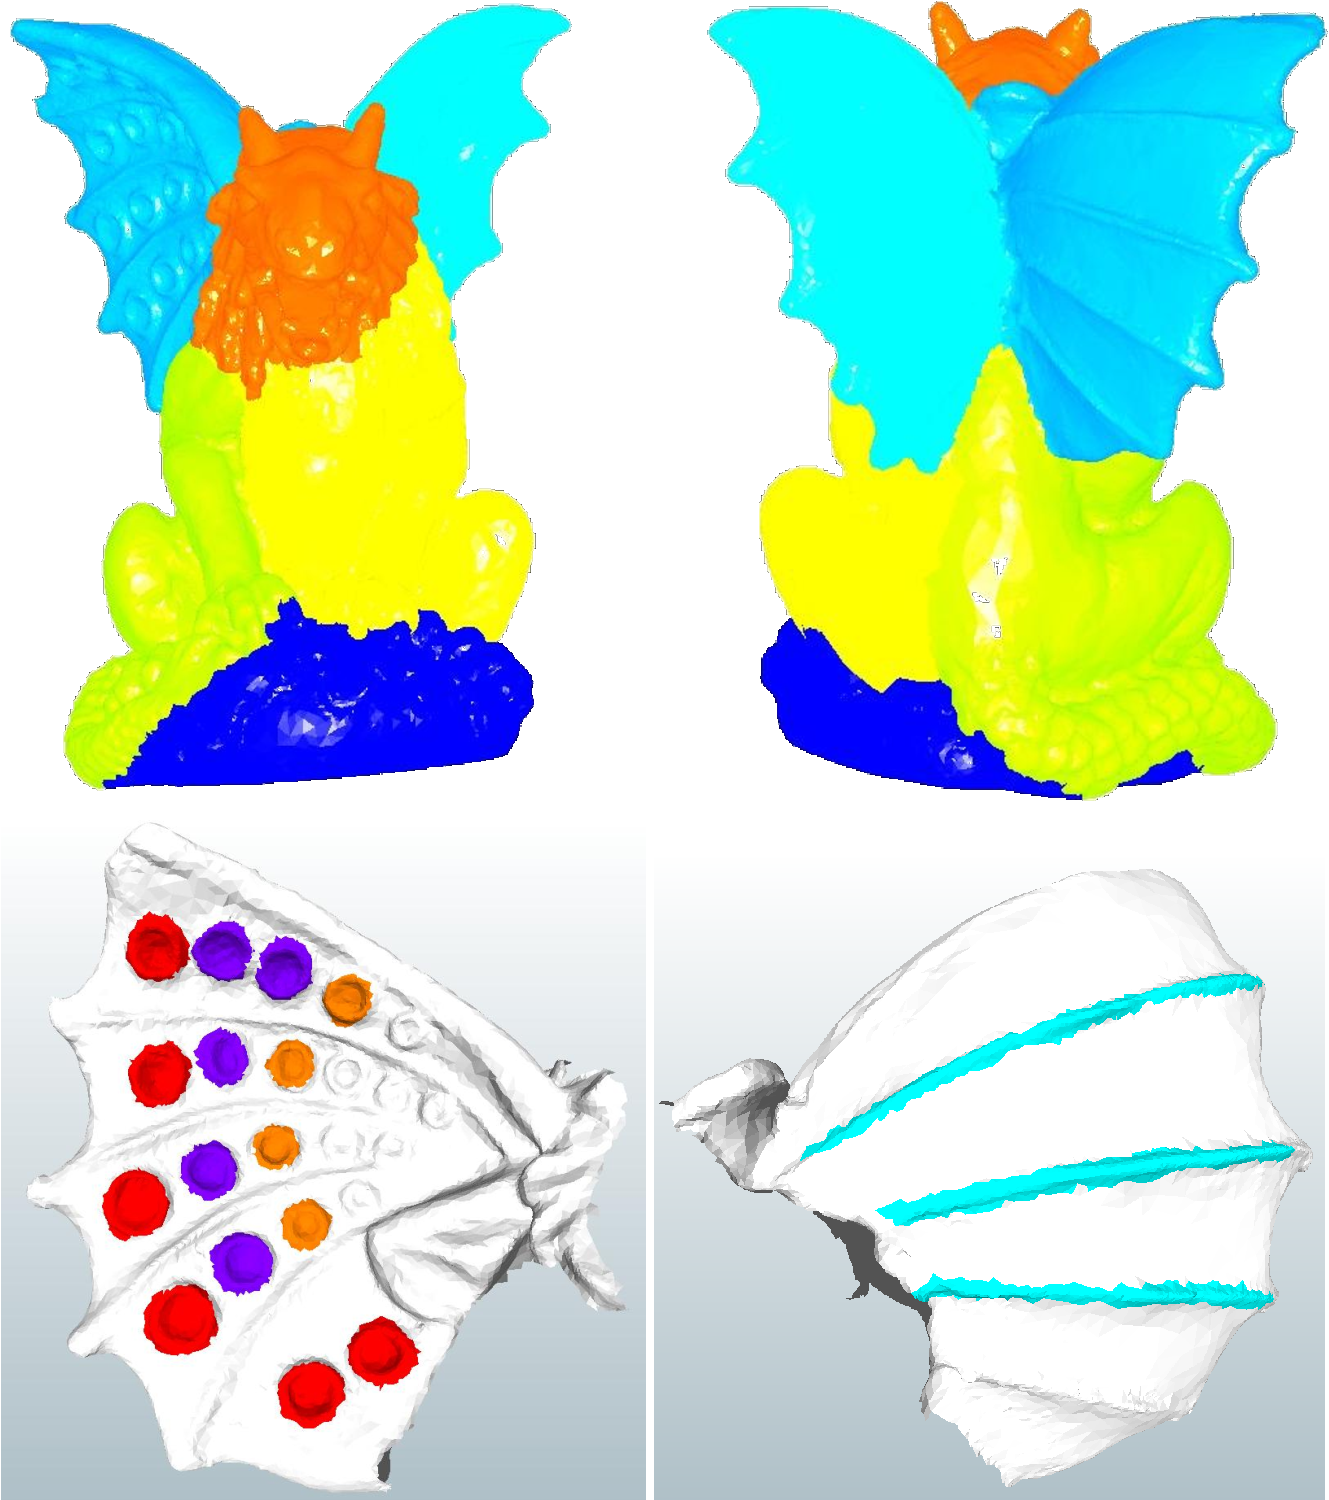
\includegraphics[width=0.95\linewidth]{figures/Gargoyl.pdf}
  \caption{Two-scale symmetries of the Gargoyle statue from two viewpoints.
  Top: At the coarse scale, two pairs of mirroring symmetry from six segmented parts are represented, with each pair being rendered by the similar color.
  Center: The results are produced by the segmentation-and-symmetry processing after 2 iterations.
  Bottom: At the fine scale, translation and rotation symmetries are detected on the left wing part for the detailed rings.}
\label{fig:Gargoyl}
\end{figure}

\section{Introduction}
\label{sec:intro}

Many objects, both man-made and natural, have approximate symmetries or self-similarities.
Finding  symmetries of meshes can be used to augment shapes with information relevant to applications such as  finite element analysis~\cite{Gellert1987}, remeshing~\cite{podolak2006}, shape simplification~\cite{pauly2008},
segmentation~\cite{Shamir2008,mitra2006,xu2009},
repair~\cite{bokeloh2009,berner2011}, and reconstruction~\cite{zabrodsky1997}.
Symmetry detection and analysis is a fundamental tool in computer graphics, computer vision and geometry processing.

Symmetries may have different definitions. In this work, we focus on generalized partial symmetry~\cite{mitra2006,berner2011} where some subsets of a shape approximately occur multiple times within the model related by combinations of translation, rotation and mirroring. Intrinsic symmetries are also considered in which case further isometric deformation is allowed between copies. This flexible definition allows symmetry detection to be more useful.

Whilst a lot of attention has been paid to both segmentation and symmetry detection, their relationship has not been fully explored.
Existing work mainly uses  symmetry detection to guide shape segmentation, as symmetry has more intrinsic semantic information than a segmentation.
However, the inverse problem, i.e.\ segmentation-based symmetry detection, has been little investigated.
All symmetry detection algorithms explicitly or implicitly use the concept that a symmetrically-related subregion of a shape is a meaningful part.
This is also the foundation of this paper, but here we employ segmentation results to benefit symmetry detection.
We further note that segmentation and symmetry detection may be used iteratively to produce hierarchical symmetry relationships in objects.

In this paper, we propose an effective method for generalized partial approximate symmetry detection.
The input shape is first segmented into multiple meaningful parts. Correspondences between each pair of parts are established using robust matching.
This is followed by a clustering stage where consistent matchings are recognized as implying a symmetry relationship between a pair of subregions.

Compared to recent graph matching algorithms~\cite{bokeloh2009,berner2011} based on salient lines our algorithm produces some robust partial symmetry detection results.
%%%RRM Please define / explain very carefully what you mean by robust and how our results are more robust
%%%ZQC The robust claims is some strong, as we could not justify it in the quanlititive evaluation by results.
For example, as shown in Figure~\ref{fig:Gargoyl}, which~\cite{berner2011} failed to handle as the paper claimed, the two-scale symmetries of the Gargoyle statue are correctly detected.
%%%RRM I am not convinced.
%%%RRM While the two wings are correct, and the green - yellow body are OK, the orange part does not look symmetric
%%%ZQC Yin is doing the iterative segmentation-symmetry refinement.
The top row shows the coarse-scale mirror symmetry detected from first-time six meaningfully segmented parts (head, left and right wing, left and right body parts, and statue base).
Two pairs of mirror symmetries (wings, body regions) have been found.
The center shows our segmentation-and-symmetry refinement results after 2 iteration, it is easy to notice that the both symmetry and segmentation are both better than the previous.
The bottom row shows fine-scale symmetry further detected when performing an analysis just on the left wing, where both  translational and rotational symmetries have been found for the detailed rings and ribs.
%%%RRM Not all rings have been found - so this is NOT robust?
%%%ZQC The other rings are so difficult to segment by current segmentation algorithm.

The rest of the paper is structured as follows. After surveying related previous work in Section 2, Section 3 describes our symmetry detection algorithm.
Section 4 demonstrates the effectiveness of our method  and provides comparisons with other approaches. Finally, Section 5 draws conclusions and discusses future work. 